\chapter{Blocks and Chains \small{\textsf{DRAFT}}}

\section{Protecting against Double Spend Attacks}

\subsection{Network Delay}

To ensure complete security of the network, all nodes must have ledgers that completely agree on the set of transactions that has happened\footnote{Interestingly, it is not necessary to require that every node agree on the order of transactions, because there is only one way to draw a construct a UTXO graph out of any valid set of transactions anyway.}. Otherwise, if two nodes have ledgers that disagree than one another, then there may be disagreements on what transactions are valid and what transactions are not. For instance, if Alice believes that she has 10 dollars left, whereas Bob believes that she only has 3, then if Alice makes a transaction with a value of 5, she will think that her own transaction is valid, whereas Bob will not, leading to a disagreement.

Using the model we have developed in class so far, it is impossible for there to be complete consensus among the ledgers. This is because we assume every  network has a network delay. Network delay, or $\Delta$, is defined as the maximum time needed for a message to reach from one honest party to every other honest party. In other words, when a honest party makes a transaction, it may take up to $\Delta$ time interval for the transaction to propagate to every other honest party. The existence of network delays allows adversaries to make a double spend attack, which is when an adversary can spend the same UTXO more than once.

\begin{figure}[]
    \centering
    \pgfplotsset{compat=1.15}
\usetikzlibrary{arrows}


\tikzset{every picture/.style={line width=0.75pt}} %set default line width to 0.75pt

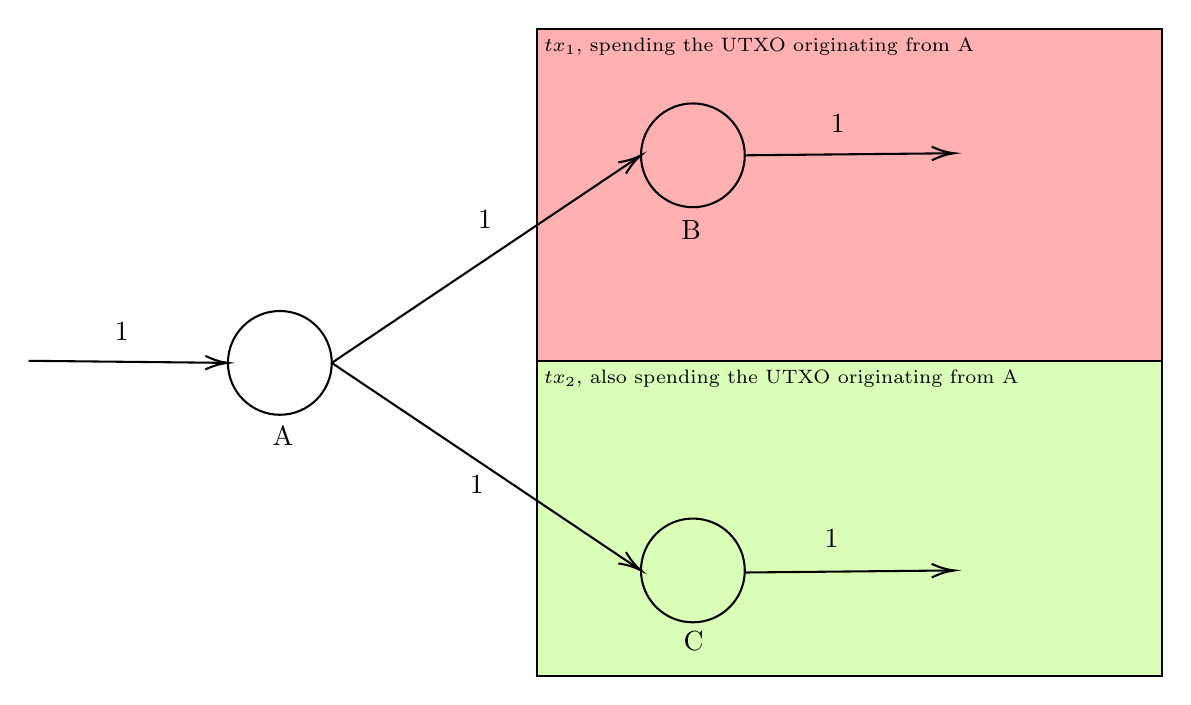
\begin{tikzpicture}[x=0.75pt,y=0.75pt,yscale=-1,xscale=1]
%uncomment if require: \path (0,373); %set diagram left start at 0, and has height of 373

%Shape: Rectangle [id:dp4222874871095379]
\draw  [fill={rgb, 255:red, 255; green, 176; blue, 176 }  ,fill opacity=1 ] (250,15) -- (551,15) -- (551,175) -- (250,175) -- cycle ;
%Shape: Rectangle [id:dp27119088832304294]
\draw  [fill={rgb, 255:red, 218; green, 255; blue, 182 }  ,fill opacity=1 ] (250,175) -- (551,175) -- (551,327) -- (250,327) -- cycle ;
%Shape: Circle [id:dp7535350871179451]
\draw   (300,76) .. controls (300,62.19) and (311.19,51) .. (325,51) .. controls (338.81,51) and (350,62.19) .. (350,76) .. controls (350,89.81) and (338.81,101) .. (325,101) .. controls (311.19,101) and (300,89.81) .. (300,76) -- cycle ;
%Shape: Circle [id:dp1786757049950185]
\draw   (101,176) .. controls (101,162.19) and (112.19,151) .. (126,151) .. controls (139.81,151) and (151,162.19) .. (151,176) .. controls (151,189.81) and (139.81,201) .. (126,201) .. controls (112.19,201) and (101,189.81) .. (101,176) -- cycle ;
%Shape: Circle [id:dp9999109102395547]
\draw   (300,276) .. controls (300,262.19) and (311.19,251) .. (325,251) .. controls (338.81,251) and (350,262.19) .. (350,276) .. controls (350,289.81) and (338.81,301) .. (325,301) .. controls (311.19,301) and (300,289.81) .. (300,276) -- cycle ;
%Straight Lines [id:da004256671229494469]
\draw    (151,176) -- (298.34,77.11) ;
\draw [shift={(300,76)}, rotate = 146.13] [color={rgb, 255:red, 0; green, 0; blue, 0 }  ][line width=0.75]    (10.93,-3.29) .. controls (6.95,-1.4) and (3.31,-0.3) .. (0,0) .. controls (3.31,0.3) and (6.95,1.4) .. (10.93,3.29)   ;
%Straight Lines [id:da6957853652663155]
\draw    (151,176) -- (298.34,274.89) ;
\draw [shift={(300,276)}, rotate = 213.87] [color={rgb, 255:red, 0; green, 0; blue, 0 }  ][line width=0.75]    (10.93,-3.29) .. controls (6.95,-1.4) and (3.31,-0.3) .. (0,0) .. controls (3.31,0.3) and (6.95,1.4) .. (10.93,3.29)   ;
%Straight Lines [id:da19761224874945627]
\draw    (350,76) -- (449,75.02) ;
\draw [shift={(451,75)}, rotate = 179.43] [color={rgb, 255:red, 0; green, 0; blue, 0 }  ][line width=0.75]    (10.93,-3.29) .. controls (6.95,-1.4) and (3.31,-0.3) .. (0,0) .. controls (3.31,0.3) and (6.95,1.4) .. (10.93,3.29)   ;
%Straight Lines [id:da5100558556413184]
\draw    (350,277) -- (449,276.02) ;
\draw [shift={(451,276)}, rotate = 179.43] [color={rgb, 255:red, 0; green, 0; blue, 0 }  ][line width=0.75]    (10.93,-3.29) .. controls (6.95,-1.4) and (3.31,-0.3) .. (0,0) .. controls (3.31,0.3) and (6.95,1.4) .. (10.93,3.29)   ;
%Straight Lines [id:da7609466290612366]
\draw    (5,175) -- (99,175.98) ;
\draw [shift={(101,176)}, rotate = 180.6] [color={rgb, 255:red, 0; green, 0; blue, 0 }  ][line width=0.75]    (10.93,-3.29) .. controls (6.95,-1.4) and (3.31,-0.3) .. (0,0) .. controls (3.31,0.3) and (6.95,1.4) .. (10.93,3.29)   ;

% Text Node
\draw (216,229) node [anchor=north west][inner sep=0.75pt]   [align=left] {1};
% Text Node
\draw (220,101) node [anchor=north west][inner sep=0.75pt]   [align=left] {1};
% Text Node
\draw (387,255) node [anchor=north west][inner sep=0.75pt]   [align=left] {1};
% Text Node
\draw (390,55) node [anchor=north west][inner sep=0.75pt]   [align=left] {1};
% Text Node
\draw (45,155) node [anchor=north west][inner sep=0.75pt]   [align=left] {1};
% Text Node
\draw (121,205) node [anchor=north west][inner sep=0.75pt]   [align=left] {A};
% Text Node
\draw (319,304) node [anchor=north west][inner sep=0.75pt]   [align=left] {C};
% Text Node
\draw (318,106) node [anchor=north west][inner sep=0.75pt]   [align=left] {B};
% Text Node
\draw (252,18) node [anchor=north west][inner sep=0.75pt]   [align=left] {{\scriptsize $tx_1$, spending the UTXO originating from A}};
% Text Node
\draw (252,178) node [anchor=north west][inner sep=0.75pt]   [align=left] {{\scriptsize $tx_2$, also spending the UTXO originating from A}};


\end{tikzpicture}
    \caption{Under our current scheme, the honest node cannot distinguish whether $tx_1$ or $tx_2$ is valid, if both are broadcasted within the network delay $\Delta$}
    \label{fig:my_label}
\end{figure}

\subsection{Double Spend}

The adversary can achieve double spending by signing and broadcasting two different transaction that spends the same UTXO. Let's call these $tx_1$ and $tx_2$ (See Figure 1). Now, notice that if it takes a maximum of $\Delta$ for a transaction to be broadcasted to every other honest note, then the honest nodes could receive these two transactions in different orders, as long as both transactions are broadcasted within a time span $\Delta$. For example, honest node $B$ could receive $tx_1$ first and validate that transaction, and then reject the $tx_2$ that comes later because an outpoint of $tx_2$ is no longer in the UTXO set. On the other hand, honest node $C$ could receive the transactions in the opposite order, and validate $tx_2$ whilst rejecting $tx_1$ as invalid. As a result, the ledgers $L_B \neq L_C$, and there will be disagreement about ownership.

% \tikzset{every picture/.style={line width=0.75pt}} %set default line width to 0.75pt

\begin{figure}[h!]
\centering
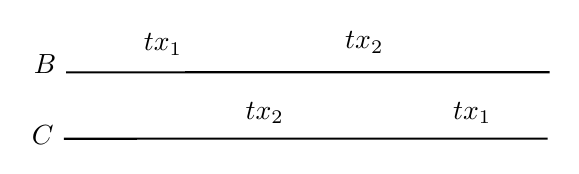
\begin{tikzpicture}[x=0.75pt,y=0.75pt,yscale=-1,xscale=1]
%uncomment if require: \path (0,300); %set diagram left start at 0, and has height of 300

%Straight Lines [id:da1698250768931009]
\draw    (95,121) -- (328,120.97) ;
%Straight Lines [id:da9907463042314588]
\draw    (94,153) -- (327,152.97) ;

% Text Node
\draw (131,101) node [anchor=north west][inner sep=0.75pt]   [align=left] {$\displaystyle tx_{1}$};
% Text Node
\draw (228,100) node [anchor=north west][inner sep=0.75pt]   [align=left] {$\displaystyle tx_{2}$};
% Text Node
\draw (280,134) node [anchor=north west][inner sep=0.75pt]   [align=left] {$\displaystyle tx_{1}$};
% Text Node
\draw (180,134) node [anchor=north west][inner sep=0.75pt]   [align=left] {$\displaystyle tx_{2}$};
% Text Node
\draw (78,111) node [anchor=north west][inner sep=0.75pt]   [align=left] {$\displaystyle B$};
% Text Node
\draw (77,145) node [anchor=north west][inner sep=0.75pt]   [align=left] {$\displaystyle C$};


\end{tikzpicture}
\caption{A possible configuration of transaction arrival times that make the protocol vulnerable to double spends, assuming both transactions reach both parties within time $\Delta$; B and C disagree whether $tx_1$ or $tx_2$ came first, i.e. which one is valid.}
\end{figure}

What are some simple solutions that could solve this double spend problem? One idea is to just cancel double spends, since no honest node would ever double spend. We would cancel both transactions if double spend occurs. However, consider the scenario where an adversary first buys an item in one transaction, and goes on to double spend the money used in that transaction after every honest node receives the first transaction. When both transactions are later cancelled, the adversary still owns that item, so the seller loses money in that case.

A second idea is to accept the first transaction that is received and cancel the second transaction. However, as previously discussed, different nodes may receive the transactions in different orders if they are broadcasted within the time span $\Delta$. As such, each node will believe that the first transaction they received is valid, and since the order of transactions cannot be guaranteed, the ledgers disagree in this case as well.

A third idea is to set up a time window. If both transactions are received within the window, then we cancel both transactions. Otherwise, we accept the first transaction and cancel the second transaction that lies outside of the time window. Ideally, the time window would allow all honest nodes to receive the first transaction, before the second transaction is then broadcasted. However, consider the scenario where the adversary broadcast the second transaction $tx_2$ at time $t$ just before the end of the time window, such that $t + \Delta$ lies outside of the time window. In this case, some nodes would recieve $tx_2$ within that time window, and other nodes would receive it outside of the time window. Hence, there will be disagreements once again.

It is clear that none of our preliminary ideas work, and to adequately defend against a double spend attack, we need to introduce the idea of a Block.

% \begin{figure}[H]
%     \centering
%     \pgfplotsset{compat=1.15}
% \pagestyle{empty}
% \definecolor{ffxfqq}{rgb}{1,0.4980392156862745,0}
% \definecolor{zzttqq}{rgb}{0.6,0.2,0}
% \definecolor{ududff}{rgb}{0.30196078431372547,0.30196078431372547,1}
% \scalebox{0.6}{
% \begin{tikzpicture}[line cap=round,line join=round,>=triangle 45,x=1cm,y=1cm]
% \begin{axis}[
% x=1cm,y=1cm,
% axis lines=none,
% ymajorgrids=false,
% xmajorgrids=false,
% xmin=-1.3128470607471872,
% xmax=20.44568941424386,
% ymin=-8.631026867350604,
% ymax=5.681622600989533,
% xtick={0,2,...,20},
% ytick={-8,-6,...,4},]
% \clip(-1.3128470607471872,-8.631026867350604) rectangle (20.44568941424386,5.681622600989533);
% \draw [->,line width=2pt] (0,0) -- (19.549029228944946,0);
% \draw [line width=2pt] (1.9776177427409318,0.8723145100091193)-- (1.9776177427409318,-1.0800645440135472);
% \draw [line width=2pt] (7.962083973549545,0.7874284641820468)-- (8.004526996463081,-1.1225075669270834);
% \draw (1.458677547283992,-1.5160681721063742) node[anchor=north west] {$ tx_1$};
% \draw (7.374021113678896,-1.5160681721063742) node[anchor=north west] {$tx_2$};
% \draw [->,line width=2pt] (6,-4) -- (12,-4);
% \draw [->,line width=2pt] (6,-4) -- (0,-4);
% \draw (5.491866342553244,-4.825351286173458) node[anchor=north west] {w};
% \begin{scriptsize}
% \draw [fill=ududff] (1.9776177427409318,0.8723145100091193) circle (2.5pt);
% \draw [fill=ududff] (1.9776177427409318,-1.0800645440135472) circle (2.5pt);
% \draw [fill=ududff] (7.962083973549545,0.7874284641820468) circle (2.5pt);
% \draw [fill=ududff] (8.004526996463081,-1.1225075669270834) circle (2.5pt);
% \end{scriptsize}
% \end{axis}
% \end{tikzpicture}}
%     \caption{Idea 3: within the window w, cancel both transactions, and outside the window w, accept the first transaction}
%     \label{fig:my_label}
% \end{figure}
\section{Blocks and Blockchains}
\subsection{Virtues of Ledgers}
There are two virtues of ledgers that should be satisfied:
\begin{itemize}
    \item \textbf{Safety:} honest parties should agree and achieve consensus.
    \item \textbf{Liveness:} transactions created by honest parties are added to the ledgers of honest parties "soon".
\end{itemize}

As observed from previous examples, double spends occur because network delays can cause disagreements in the arrival time of different transactions. If somehow transactions could only be created in intervals greater than the network delay parameter $\Delta$, there would be no disagreements because each transaction would have already been broadcasted to all honest parties before the next one gets broadcasted. This gives rise to safety. However, requiring such a delay between transactions means that there will be less transactions being broadcasted every time period, and as such it may be the case that the liveness property is not satisfied. This presents a tradeoff between safety and liveness: as $\Delta$ increases, there is less certainty for liveness to be guaranteed.

\subsection{Blocks}

One way to satisfy both the virtues of safety and liveness is to group multiple transactions together and then broadcast them as "blocks", rather than individually. Each block, denoted $\Bar{x} = (tx_1, tx_2, \dots)$, contains a sequence of transactions in any order that respects the topological sorting of the corresponding UTXO graph.

In this model, double spends can only occur if the two transactions that creates the double spend exist in 2 different blocks that arrives in different order to different honest parties, similar to the previous example with transactions. If the two double spending transactions appeared within the same block, then there is no valid UTXO graph for the transactions of that block, and so the entire block is invalid. If the two double spending transactions appear in two blocks that are further than $\Delta$ apart, then the first transaction would have been validated by all honest parties, and so the second transaction fails to double spend.

Hence, all we need to do to ensure protection against double spending is to ensure that each  \textbf{block}—rather than each transaction—is rare, which preserves safety  while ensuring a higher level of liveness.

\begin{figure}[H]
    \centering
    \pgfplotsset{compat=1.15}


\tikzset{every picture/.style={line width=0.75pt}} %set default line width to 0.75pt

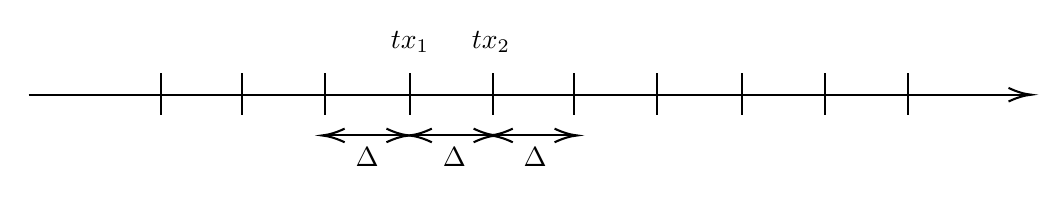
\begin{tikzpicture}[x=0.75pt,y=0.75pt,yscale=-1,xscale=1]
%uncomment if require: \path (0,300); %set diagram left start at 0, and has height of 300

%Straight Lines [id:da9017954087564621]
\draw    (97,110.2) -- (578,110.2) ;
\draw [shift={(580,110.2)}, rotate = 180] [color={rgb, 255:red, 0; green, 0; blue, 0 }  ][line width=0.75]    (10.93,-3.29) .. controls (6.95,-1.4) and (3.31,-0.3) .. (0,0) .. controls (3.31,0.3) and (6.95,1.4) .. (10.93,3.29)   ;
%Straight Lines [id:da09295967444550124]
\draw    (160.73,99.83) -- (160.73,119.83) ;
%Straight Lines [id:da22506827825676345]
\draw    (199.73,99.83) -- (199.73,119.83) ;
%Straight Lines [id:da6864589596901391]
\draw    (239.73,99.83) -- (239.73,119.83) ;
%Straight Lines [id:da3375627515094475]
\draw    (280.73,99.83) -- (280.73,119.83) ;
%Straight Lines [id:da2711314265282385]
\draw    (320.73,99.83) -- (320.73,119.83) ;
%Straight Lines [id:da9006595698348807]
\draw    (359.73,99.83) -- (359.73,119.83) ;
%Straight Lines [id:da2941667702377173]
\draw    (399.73,99.83) -- (399.73,119.83) ;
%Straight Lines [id:da4637768077817921]
\draw    (440.73,99.83) -- (440.73,119.83) ;
%Straight Lines [id:da15003143298927957]
\draw    (480.73,99.83) -- (480.73,119.83) ;
%Straight Lines [id:da7785431556267932]
\draw    (520.73,99.83) -- (520.73,119.83) ;
%Straight Lines [id:da07195865234652721]
\draw    (259.29,129.83) -- (278.29,129.83) ;
\draw [shift={(280.29,129.83)}, rotate = 180] [color={rgb, 255:red, 0; green, 0; blue, 0 }  ][line width=0.75]    (10.93,-3.29) .. controls (6.95,-1.4) and (3.31,-0.3) .. (0,0) .. controls (3.31,0.3) and (6.95,1.4) .. (10.93,3.29)   ;
%Straight Lines [id:da13395559951976144]
\draw    (259.29,129.83) -- (240.29,129.83) ;
\draw [shift={(238.29,129.83)}, rotate = 360] [color={rgb, 255:red, 0; green, 0; blue, 0 }  ][line width=0.75]    (10.93,-3.29) .. controls (6.95,-1.4) and (3.31,-0.3) .. (0,0) .. controls (3.31,0.3) and (6.95,1.4) .. (10.93,3.29)   ;
%Straight Lines [id:da3690305468137254]
\draw    (301.29,129.83) -- (320.29,129.83) ;
\draw [shift={(322.29,129.83)}, rotate = 180] [color={rgb, 255:red, 0; green, 0; blue, 0 }  ][line width=0.75]    (10.93,-3.29) .. controls (6.95,-1.4) and (3.31,-0.3) .. (0,0) .. controls (3.31,0.3) and (6.95,1.4) .. (10.93,3.29)   ;
%Straight Lines [id:da6757384410639338]
\draw    (301.29,129.83) -- (282.29,129.83) ;
\draw [shift={(280.29,129.83)}, rotate = 360] [color={rgb, 255:red, 0; green, 0; blue, 0 }  ][line width=0.75]    (10.93,-3.29) .. controls (6.95,-1.4) and (3.31,-0.3) .. (0,0) .. controls (3.31,0.3) and (6.95,1.4) .. (10.93,3.29)   ;
%Straight Lines [id:da008698697312877313]
\draw    (340.29,129.83) -- (359.29,129.83) ;
\draw [shift={(361.29,129.83)}, rotate = 180] [color={rgb, 255:red, 0; green, 0; blue, 0 }  ][line width=0.75]    (10.93,-3.29) .. controls (6.95,-1.4) and (3.31,-0.3) .. (0,0) .. controls (3.31,0.3) and (6.95,1.4) .. (10.93,3.29)   ;
%Straight Lines [id:da5776529929797669]
\draw    (340.29,129.83) -- (321.29,129.83) ;
\draw [shift={(319.29,129.83)}, rotate = 360] [color={rgb, 255:red, 0; green, 0; blue, 0 }  ][line width=0.75]    (10.93,-3.29) .. controls (6.95,-1.4) and (3.31,-0.3) .. (0,0) .. controls (3.31,0.3) and (6.95,1.4) .. (10.93,3.29)   ;

% Text Node
\draw (253,134.4) node [anchor=north west][inner sep=0.75pt]    {$\Delta $};
% Text Node
\draw (295,134.4) node [anchor=north west][inner sep=0.75pt]    {$\Delta $};
% Text Node
\draw (334,134.4) node [anchor=north west][inner sep=0.75pt]    {$\Delta $};
% Text Node
\draw (270,78.4) node [anchor=north west][inner sep=0.75pt]    {$tx_{1}$};
% Text Node
\draw (309,78.4) node [anchor=north west][inner sep=0.75pt]    {$tx_{2}$};


\end{tikzpicture}

    \caption{In an ideal scenario, each blocks are broadcasted exactly $\Delta$ away from each other, so in a double spend we can always accept $tx_1$ and reject $tx_2$}
    \label{fig:my_label}
\end{figure}

\subsection{Proof of Work and Mining}
To ensure that the ability to create blocks is rare (i.e. that one can only be created after $\Delta$ has passed since the last block), we devise a scheme to issue rare tickets for creating a block. To do so, we will introduce the concept of Proof of Work.

% \subsection{Blocks and Proof of Work}

% There are two virtues of ledgers. The first is safety, which means that ledgers of honest parties should agree and reach consensus. The second is liveness, which means a transaction issued by an honest party should make it into honest ledgers soon.

% As observed from previous examples, a reason why double spends are difficult to deal with is because two transactions can be broadcasted within a short time span. If only one transaction can be broadcasted every $\Delta$, then the problem of double spends is easy to deal with because each node would receive transactions in the same order. However, the tradeoff in this case would slow throughput which can prevent the liveness property from being satisfied.

% This motivates the use of blocks to store transactions. A block stores a bundled sequence of transactions, denoted as $\Bar{x}$. We want one new block to be broadcasted roughly every $\Delta$. To ensure this time span, we will introduce the Proof-of-Work Equation.

\begin{definition}[Proof-of-Work Equation]
  $H(B) \leq T$
  \footnote{This scheme was derived in 1993 by Cynthia Dwork and Moni Naor in the seminal paper "Pricing via Processing
or Combatting Junk Mail".}
\end{definition}

Here, $T$ is called the target. In order to solve the Proof-of-Work equation, one would have to find a value of $B$ such that $H(B) \leq T$.

\begin{definition}[Random Oracle Model]
  Output of $H$ is distributed uniformly at random.
\end{definition}

Under the Random Oracle Assumption, notice that the time it would take to find a bruteforce solution to a Proof-of-Work equation depends on the value of $T$. When $T$ is larger, it would be easier to find $B$ such that $H(B) \leq T$, and vice versa. In particular, $Pr[H(B) \leq T] = \frac{T}{2^{\kappa}}$ for any arbitrary $B$.

In the network, $T$ is fixed and hard-coded for honest parties. The value is chosen such that the time it takes for a node in the network to find a solution to the Proof-of-Work equation is around $\Delta$.

Now, notice that if we allow honest parties to pick whatever $B$ they want, then as soon as the first valid value of $B$ is found, each node can just trivially reuse that value instantaneously, and safety is lost again. As such, in the network, we require that $B = \delta||\Bar{x}||ctr$, where $||$ means concatenation and where $\delta$ is the hash of the previous block $H(B')$. Both $\delta$ and $\Bar{x}$ are fixed, and $ctr$ is a number to be found that solves the Proof-of-Work equation. In other words, when nodes are trying to solve the Proof-of-Work equation, they are trying different values of $ctr$ until finding a satisfactory one. The time it takes the first node to find a satisfactory $ctr$ for their block will be around $\delta$. The process of finding a bruteforce solution to the Proof-of-Work equation is called mining.

\subsection{Blockchains}

The previous block hash, $\delta$, is a part of $B$ because we want to ensure "freshness", which means that only blocks that are recently created should be able to be broadcasted. Consider the scenario where an adversary mines multiple blocks, but does not broadcast them immediately. Then, at a later point in time, the adversary broadcast all of these blocks at the same time. Since there is not a $\Delta$ interval between the time these blocks are broadcasted, the problem of double spend arises again. There could be disagreements in the ledgers of the honest nodes. In order to prevent this, we require each block to point to the most recent known block. By including $\delta$ as a part of $B$, we ensure that blocks that were mined beforehand are no longer valid, since the adversary could not have predicted $\delta$ before the most recent block was broadcasted. As a result, we can guarantee that blocks will be roughly be broadcasted in regular time intervals. Since blocks are all connected to each other in this way, this chain of block is called the \emph{blockchain}.


\subsection{Genesis Block}

The Genesis Block is the first block in a blockchain. It contains real world data to anchor time, in order to ensure that it is impossible to pre-mine. If the hash of the Genesis Block is known before it is broadcasted, then the adversary could pre-mine multiple blocks beforehand (before the network is even available to the rest of the world). Then, when the Genesis Block is broadcasted, the adversary would be able to broadcast multiple blocks within a short time span. Hence, it is necessary for the Genesis Block to contain real world data to anchor time. For example, Bitcoin genesis block quotes the January 3  2009 The Times headline.

\begin{figure}[H]
    \centering
    \pgfplotsset{compat=1.15}



\tikzset{every picture/.style={line width=0.75pt}} %set default line width to 0.75pt

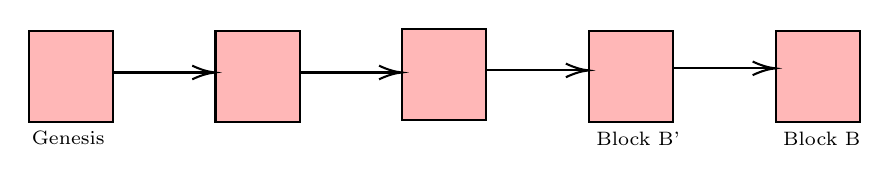
\begin{tikzpicture}[x=0.75pt,y=0.75pt,yscale=-1,xscale=1]
%uncomment if require: \path (0,165); %set diagram left start at 0, and has height of 165

%Shape: Rectangle [id:dp6459725379232777]
\draw  [fill={rgb, 255:red, 255; green, 183; blue, 183 }  ,fill opacity=1 ] (132,36) -- (172.53,36) -- (172.53,80.09) -- (132,80.09) -- cycle ;
%Shape: Rectangle [id:dp7451543919622989]
\draw  [fill={rgb, 255:red, 255; green, 183; blue, 183 }  ,fill opacity=1 ] (222,36) -- (262.53,36) -- (262.53,80.09) -- (222,80.09) -- cycle ;
%Shape: Rectangle [id:dp4942977774139823]
\draw  [fill={rgb, 255:red, 255; green, 183; blue, 183 }  ,fill opacity=1 ] (312,35) -- (352.53,35) -- (352.53,79.09) -- (312,79.09) -- cycle ;
%Shape: Rectangle [id:dp8525801453597799]
\draw  [fill={rgb, 255:red, 255; green, 183; blue, 183 }  ,fill opacity=1 ] (402,36) -- (442.53,36) -- (442.53,80.09) -- (402,80.09) -- cycle ;
%Shape: Rectangle [id:dp16781400895186005]
\draw  [fill={rgb, 255:red, 255; green, 183; blue, 183 }  ,fill opacity=1 ] (492,36) -- (532.53,36) -- (532.53,80.09) -- (492,80.09) -- cycle ;
%Straight Lines [id:da27296871485376917]
\draw    (172.73,56.09) -- (219.73,56.09) ;
\draw [shift={(221.73,56.09)}, rotate = 180] [color={rgb, 255:red, 0; green, 0; blue, 0 }  ][line width=0.75]    (10.93,-3.29) .. controls (6.95,-1.4) and (3.31,-0.3) .. (0,0) .. controls (3.31,0.3) and (6.95,1.4) .. (10.93,3.29)   ;
%Straight Lines [id:da8965885073779516]
\draw    (262.73,56.09) -- (309.73,56.09) ;
\draw [shift={(311.73,56.09)}, rotate = 180] [color={rgb, 255:red, 0; green, 0; blue, 0 }  ][line width=0.75]    (10.93,-3.29) .. controls (6.95,-1.4) and (3.31,-0.3) .. (0,0) .. controls (3.31,0.3) and (6.95,1.4) .. (10.93,3.29)   ;
%Straight Lines [id:da16101344176853494]
\draw    (352.73,55.09) -- (399.73,55.09) ;
\draw [shift={(401.73,55.09)}, rotate = 180] [color={rgb, 255:red, 0; green, 0; blue, 0 }  ][line width=0.75]    (10.93,-3.29) .. controls (6.95,-1.4) and (3.31,-0.3) .. (0,0) .. controls (3.31,0.3) and (6.95,1.4) .. (10.93,3.29)   ;
%Straight Lines [id:da6603043582779935]
\draw    (442.73,54.09) -- (489.73,54.09) ;
\draw [shift={(491.73,54.09)}, rotate = 180] [color={rgb, 255:red, 0; green, 0; blue, 0 }  ][line width=0.75]    (10.93,-3.29) .. controls (6.95,-1.4) and (3.31,-0.3) .. (0,0) .. controls (3.31,0.3) and (6.95,1.4) .. (10.93,3.29)   ;

% Text Node
\draw (132,83.09) node [anchor=north west][inner sep=0.75pt]   [align=left] {{\scriptsize Genesis}};
% Text Node
\draw (404,83.09) node [anchor=north west][inner sep=0.75pt]   [align=left] {{\scriptsize Block B'}};
% Text Node
\draw (494,83.09) node [anchor=north west][inner sep=0.75pt]   [align=left] {{\scriptsize Block B}};


\end{tikzpicture}

    \caption{To mine block B, the miner runs the Proof of Work Equation with B = $H(B')||\Bar{x}||ctr$}
    \label{fig:my_label}
\end{figure}


\subsection{Honest Party Block Generation Algorithm}

Putting it all together, an honest party (which we can assume to be every honest node in the network for now) follows the following algorithm to create a valid block. First, it collects any amount of transactions from the network and add them to a mempool, which is a set of validated but unconfirmed transactions \footnote{The number of transactions it collects will be formalized later}. Then, it writes $B = \delta||\Bar{x}||ctr$, and then solves the Proof-of-Work Equation. In other words, it finds a value of ctr (which is also known as the nonce) such that $H(B) \leq T$. If the honest party is successful, it will broadcast the mined block to the network. Otherwise, if another block has been found and received by the honest party first, it will validate the new block, update it's UTXO by removing all the transactions that were spent in the newest block, and update the freshest block in its memory. As such, $B$ would necessarily change, and the honest party will have to solve a new Proof-of-Work equation.

%TODO: maybe rewrite using algorithms package?
